\documentclass[12pt]{article}
\usepackage{epsfig}
\usepackage{graphicx}
\usepackage{a4}
\usepackage{amsmath}
\usepackage{latexsym}
\usepackage{cite}
%\usepackage{draftwatermark}
\usepackage{lineno}
\usepackage{xspace}
%\usepackage{chngcntr}


\usepackage{color}
\usepackage{colordvi}

\graphicspath{{Pics/}}
\DeclareGraphicsExtensions{.eps,.ps}

\textheight 22.0cm \textwidth 16.5cm
\oddsidemargin -0.1cm \evensidemargin -0.1cm

\usepackage{pslatex}
\usepackage[latin1]{inputenc}
\usepackage[T1]{fontenc}
\usepackage{amssymb}
\usepackage{url}

\newcommand{\msbar}{$\overline{\text{MS}}\, $\xspace}

%
\linenumbers
%
% ----------------------------------------------------------------------------------------------
%
\begin{document}

\begin{titlepage}
\noindent
Draft 1.5  \hfill 08 November 2019\\
\\
DESY AA-BBB %\hfill  2019\\
\\

\vspace{1.3cm}

\begin{center}
  {\bf 

\large

Improved constraints on parton distributions using LHCb, ALICE and HERA heavy-flavour measurements and implications for the predictions for prompt atmospheric neutrino fluxes. 
  }
  \vspace{1.5cm}

  {\large
    PROSA Collaboration
  }\\

  \vspace{1.2cm}

\end{center}
 %\input{authors.tex}  
  \vspace{2.4cm}
\begin{center}
\large
{\bf Abstract}
\vspace{-0.2cm}
\end{center}
%%
The impact of measurements of heavy-flavour production in deep inelastic ep scattering and
in pp collisions on parton distribution functions is studied in a QCD analysis at next-to-leading order. 
Recent combined results of inclusive and heavy-flavour production cross sections in deep inelastic scattering at HERA are 
investigated together with heavy-flavour production measurements at the LHC. Differential cross sections of charm- and 
beauty-hadron production measured by the LHCb collaboration at the centre of mass energies of 5, 7 and 13 TeV as well 
as the recent measurements of the ALICE experiment at the centre of mass energies of 5 and 7 TeV are explored. 
These data impose additional constraints on the gluon and the sea-quark distributions at low partonic fractions
$x$ of the proton momentum, down to $x\approx10^{-6}$. The impact of the resulting parton distribution function in the predictions for the prompt atmospheric neutrino fluxes is studied.


%%
\vfill
\end{titlepage}


%
% ----------------------------------------------------------------------------------------------
%
\newpage

\section{Introduction}
\label{sect:intro}

The fundamental structure of the nucleon is described by the theory of strong interactions, quantum chromodynamics (QCD).
In the collinear factorisation, the nucleon structure is expressed in terms of parton distribution functions (PDFs), defined 
as probability densities for partons to carry a fraction $x$ of the nucleon momentum at a factorisation scale $\mu_f$. While the 
scale evolution of the PDFs is calculated in perturbative QCD (pQCD) using the DGLAP equations~\cite{Dokshitzer:1977sg,Gribov:1972ri,Altarelli:1977zs,Curci:1980uw,Furmanski:1980cm,Moch:2004pa,Vogt:2004mw}, the 
$x$-dependence must be constrained from the experimental measurements. The constraining power of experimental data 
on particular parton distribution is to large extent defined by the acceptance of the experiment. Measurements of 
neutral current (NC) and charged current (CC) cross sections in deep inelastic scattering (DIS) at HERA probe the $x$-range of $10^{-4}<x<10^{-1}$, impose most significant constraints on the light quark PDFs and probe the gluon distribution via scaling violations. Additional constraints on the flavour separation of the quark sea and on the gluon distribution at low and high $x$ are obtained by using the measurements at fixed target experiments and in proton-(anti)proton collisions. Heavy-flavour production in proton-proton ($pp$) collisions at the LHC is dominated by the gluon-gluon fusion, therefore corresponding measurements probe the gluon distribution directly. The measurements of forward charm~\cite{Aaij:2013mga} and beauty~\cite{Aaij:2013noa} production by the LHCb experiment at the centre-of-mass energy $\sqrt{s}=7$ TeV were used for the first time by the PROSA collaboration~\cite{Zenaiev:2015rfa} to improve constraints on the gluon distribution at $5 \times 10^{-6}< x < 10^{-4}$, in the region hardly covered by any other data to that date. The resulting PDFs (referred in the following as PROSA 2015) were further used to investigate the uncertainties in the predictions of prompt neutrino fluxes in the atmosphere~\cite{Garzelli:2016xmx}.       

Recent improvements in precision of HERA measurements, new experimental data on heavy flavour production at the LHC at 
different $\sqrt{s}$, together with new developments in the theory and improvements of the phenomenological tools, offer 
possibilities for stronger constraints on the gluon distribution at low $x$. These improvements in experimental measurements 
and the theory are explored in the QCD analysis presented in this paper, which updates the earlier PDF result~\cite{Zenaiev:2015rfa}. The results, referred to as PROSA 2019, are used to update the predictions for the prompt atmospheric neutrino fluxes. 


\section{Input data sets and used theory predictions}
\label{sec:qcdanalysis}

The main objective of the present QCD analysis is to demonstrate the constraining power of the updated measurements of 
heavy-flavour production in DIS and $pp$ collisions for the determination of the PDFs of the proton. 
The QCD analysis is performed at next-to-leading order (NLO) using the xFitter framework~\cite{Alekhin:2014irh}. 
The updated combinations of the inclusive DIS cross sections~\cite{Abramowicz:2015mha} and of charm and beauty production cross sections~\cite{H1:2018flt} are used together with the measurements of charm and beauty hadroproduction in $pp$ scattering at the LHC. The latter include the measurements of charm hadroproduction by the LHCb collaboration at $\sqrt{s}$ = 5 TeV~\cite{Aaij:2016jht}, 7 TeV~\cite{Aaij:2013mga} and 13 TeV~\cite{Aaij:2015bpa}, and by ALICE at $\sqrt{s}$ = 5 TeV~\cite{Acharya:2019mgn} and 7 TeV~\cite{Acharya:2017jgo}. The measurements of beauty hadroproduction by the LHCb at $\sqrt{s}$ = 7 TeV~\cite{Aaij:2013noa} are also used.

The cross sections measured by the LHCb and ALICE in each $p_T$ range are normalised in rapidity $y$, $\frac{{\rm d}^2\sigma}{{\rm d}y{\rm d}p_T} / (\frac{{\rm d}^2\sigma}{{\rm d}y{\rm d}p_T})_{0}$. Here, $\left(\frac{{\rm d}^2\sigma}{{\rm d}y{\rm d}p_T}\right)_{0}$ is the cross section in the central LHCb rapidity bin, $3 < y < 3.5$. 
Note that ALICE measurements at $|y| < 0.5$ are normalised to the LHCb cross section measurement in $3 < y < 3.5$. 
The advantage of using the normalised cross section, demonstrated in the earlier PROSA analysis~\cite{Zenaiev:2015rfa}, 
is a significant reduction of the scale dependence in the theoretical prediction,  while retaining the sensitivity to 
the PDFs. 

In the presented QCD analysis, bin-to-bin correlations in the input measurements are taken into account as described in the following. The treatment of correlated experimental uncertainties for the HERA data follows that of the original publications~\cite{Abramowicz:2015mha,H1:2018flt}.
 
The correlated uncertainties in the ALICE and LHCb measurements reported in original publications~\cite{Aaij:2016jht, Aaij:2013mga, Aaij:2015bpa, Acharya:2019mgn, Acharya:2017jgo, Aaij:2013noa} and listed in the respective tables as exact uncertainty values in each kinematic bin in $p_T$ and $y$, 
are treated as fully correlated, and the uncorrelated uncertainties are obtained by subtracting the correlated ones from the 
total uncertainties, in quadrature. Because of this treatment of systematics, most of these correlated systematic uncertainties cancel in the calculation of the normalised cross sections. In case of the LHCb cross section ratio measurements, the uncertainties cancel completely. The systematic uncertainties, reported as error intervals, see e.g. Table~(2) of Ref.~\cite{Aaij:2016jht}, are assumed uncorrelated, since no details about their size in individual $p_T$ and $y$ bins are provided. 
For different final state measurements within one experiment, the tracking and luminosity uncertainties are treated as correlated. 
Furthermore, all experimental uncertainties are treated as uncorrelated among measurements at different centre-of-mass energies. 
The uncorrelated uncertainties in the normalised cross sections $\frac{{\rm d}\sigma}{{\rm d}y_0}$ are propagated as correlated uncertainties to the respective complementary rapidity bins.
It is worthwhile to note, that the details of the experimental uncertainties and their correlations in each individual kinematic range is of great importance and therefore most detailed information about the systematic correlations in the experimental measurement is required.

In the presented QCD analysis, the scale evolution of partons is calculated through DGLAP equations at NLO, as implemented in 
the QCDNUM programme~\cite{openqcdrad}.  
The description of HERA data in PDF fits improves in the kinematic range of small $x$ and low $Q^2$, by including higher twist effects~\cite{Accardi:2016ndt,Alekhin:2017kpj}
or, alternatively, small $x$ resummation~\cite{Ball:2017otu,Abdolmaleki:2018jln}. 
These upgrades are left for future analyses, once all necessary theoretical ingredients have become available. 

The theoretical predictions for the heavy-quark and inclusive HERA data are obtained using OPENQCDRAD~\cite{openqcdrad} code in the 
fixed-flavour-number scheme (FFNS) with the three active flavours in the proton, following the Ref.~\cite{H1:2018flt}. 
Similar to the earlier PROSA analysis~\cite{Zenaiev:2015rfa}, the theoretical predictions for the fully differential 
heavy-quark hadroproduction in $pp$ collisions, available at NLO in FFNS, are used. These are calculated using 
the MNR code, with the single-particle inclusive distributions computed using the pole mass scheme for the heavy quarks, 
and translated into the \msbar scheme expressions using the \msbar mass $m_Q(m_Q)$ and following the Ref.~\cite{Dowling:2013baa}.
The \msbar mass scheme is then consistently used in the calculations for all used processes.

The factorisation and renormalisation scales are chosen to be $Q$ for the inclusive DIS, and $\mu_r = \mu_f = \sqrt{Q^2 + 4m_Q(m_Q)^2}$ for the heavy quark production in DIS, respectively, with $m_Q(m_Q)$ representing the heavy-quark mass in the \msbar scheme. 
For heavy quark production in $pp$ collision, $\mu_r = \mu_f = \sqrt{4m_Q(m_Q)^2+p_T^2}$ is assumed. 

The calculations for the heavy quark hadroproduction are supplemented with phenomenological non-perturbative fragmentation 
functions to describe the transition of heavy quarks into hadrons. The fragmentation of charm quarks into $D$-mesons is 
described by the Kartvelishvili function $D_Q(z) \propto z^{\alpha_K}(1-z)$ 
with $\alpha_K = 4.4 \pm 1.7$ as measured at HERA~\cite{Aaron:2008ac,Chekanov:2008ur}, 
and for the fragmentation of beauty quarks $\alpha_K = 11 \pm 3$ is used as measured at LEP~\cite{Nason:1999zj}, following 
the previous PROSA analysis~\cite{Zenaiev:2015rfa}.
Studies of the uncertainties related to the fragmentation in \cite{Alekhin:2012un} 
for a determination of the charm-quark mass in the \msbar scheme from
deep inelastic scattering at HERA data have shown that the dominant effect is
captured by varying $\alpha_K$ within its uncertainties. 
This treatment of charm quark fragmentation is independent of choice of a particular renormalisation scheme for the heavy quark mass. 
The latter is needed in a determination of the initial condition for the perturbative heavy quark fragmentation
function, which is known to NNLO~\cite{Melnikov:2004bm}.
The subsequent range of evolution in the case of charm quark fragmentation
into $D$-mesons from the scale of hadronisation to scales of order of the
charm quark mass is very short, so that the modelling with the non-perturbative Kartvelishvili function $D_Q(z)$ is justified.

The main QCD analysis is performed in the FFNS and the sensitivity of the heavy quark measurements to the PDFs and to the masses 
of the charm and beauty quarks is fully explored by treating $m_c(m_c)$ and $m_b(m_b)$ as free parameters in the fit.
The fit is also performed in the variable flavour number scheme (VFNS) to allow for incorporation in Shower Monte Carlo event generators and applications in e.g. 
underlying event tuning at the LHC.


\section{PDF parametrisation}
\label{sec:pdfparam}

The PDFs are parametrised at the starting evolution scale of $\mu^2_{f0} = 1.9$~GeV$^2$, similar as in Ref.~\cite{Abramowicz:2015mha} and Ref.~\cite{Bonvini:2019wxf}, as follows:
\begin{equation}\begin{aligned}
xg(x) &= A_{g} x^{B_{g}}\,(1-x)^{C_{g}}\, (1 + F_{g} {\log x}),\\
xu_\mathrm{v}(x) &= A_{u_\mathrm{v}}x^{B_{u_\mathrm{v}}}\,(1-x)^{C_{u_\mathrm{v}}}\,(1+E_{u_\mathrm{v}}x^2) ,\\
xd_\mathrm{v}(x) &= A_{d_\mathrm{v}}x^{B_{d_\mathrm{v}}}\,(1-x)^{C_{d_\mathrm{v}}},\\
x\overline{\mathrm{U}}(x)&= A_{\overline{\mathrm{U}}}x^{B_{\overline{\mathrm{U}}}}\, (1-x)^{C_{\overline{\mathrm{U}}}}\, (1+D_{\overline{\mathrm{U}}}x), \\
x\overline{\mathrm{D}}(x)&= A_{\overline{\mathrm{D}}}x^{B_{\overline{\mathrm{D}}}}\, (1-x)^{C_{\overline{\mathrm{D}}}}.
\end{aligned}
\label{eq:dv}
\end{equation}

Here, $xg(x)$, $xu_{\mathrm{v}}(x)$ and $xd_{\mathrm{v}}(x)$ represent the gluon, up and down valence quark distributions, respectively. The sea quark distribution is defined as $x\Sigma(x)=x\overline{u}(x)+x\overline{d}(x)+x\overline{s}(x)$, with $x\overline{u}(x)$, $x\overline{d}(x)$, and $x\overline{s}(x)$ denoting the up, down, and strange antiquark distributions, respectively.
For the up- and down-type antiquark distributions, $x\overline{\mathrm{U}}(x)$ and $x\overline{\mathrm{D}}(x)$, relations $x\overline{\mathrm{U}}(x) = x\overline{u}(x)$ and $x\overline{\mathrm{D}}(x) = x\overline{d}(x) + x\overline{s}(x)$  are assumed.
The normalisation parameters $A_{u_{\mathrm{v}}}$, $A_{d_\mathrm{v}}$, and $A_{g}$ are determined by the QCD sum rules.
The strangeness fraction $f_{s} = x\overline{s}/( x\overline{d} + x\overline{s})$ is fixed to
$f_{s}=0.4$ as in the HERAPDF2.0 analysis~\cite{Abramowicz:2015mha}.
Additional constraints $B_{\overline{\mathrm{U}}} = B_{\overline{\mathrm{D}}}$ and $A_{\overline{\mathrm{U}}} = A_{\overline{\mathrm{D}}}(1 - f_{s})$ are imposed to ensure the same normalisation for the $x\overline{u}$ and $x\overline{d}$ distributions as $x \to 0$.
The term $F_g\log x$ was proposed in~\cite{Bonvini:2019wxf} to provide a more flexible functional form at low $x$.

The predicted and measured cross sections together with their corresponding uncertainties are used to build a global $\chi^2$, minimised to determine the initial PDF
parameters. The $\chi^2$ definition follows that of Eq.~(32) in Ref.~\cite{Abramowicz:2015mha}. In the minimisation, performed 
using the MINUIT package~\cite{James:1975dr}, the experimental uncertainties in the heavy-quark normalised cross 
sections are treated as additive, and the treatment of the experimental uncertainties for the HERA DIS data follows 
the prescription given in Ref.~\cite{Abramowicz:2015mha}.

%The parameters in Eq.~(\ref{eq:dv}) are selected by first setting all $D$ and $E$ parameters to zero. 
The parameters in Eq.~(\ref{eq:dv}) are selected by first parametrising each PDF as
\begin{equation}
xf(x) = Ax^B(1-x)^C(1+Dx+Ex^2)
\label{eq:de}
\end{equation}
and setting all $D$ and $E$ parameters to zero.
Additional parameters in each resulting PDFs are included in the fit one at a time. 
The improvement in $\chi^2$ of the fits is monitored and the procedure is stopped when no further improvement is observed. The inclusion of the $F_{g}$ parameter does not lead to significant change in $\chi^2$, in particular, its fitted value is consistent with $0$ within uncertainty, however the variation of $F_{g}$ significantly affects the fit uncertainties.

To ensure that the gluon PDF at low $x$ is not over-constrained in the fit, different functional forms in the parametrisation were tested, as used in the ABMP16~\cite{Alekhin:2017kpj}, CT14~\cite{Dulat:2015mca}, HERAPDF2.0~\cite{Abramowicz:2015mha}, MMHT2014~\cite{Harland-Lang:2014zoa} and Bonvini-Giuli (BG)~\cite{Bonvini:2019wxf} PDF fits:

\begin{equation}
\begin{aligned}
\textrm{ABMP16:}~~~~~~ &xg(x)=A (1 - x)^b x^{a (1 + \gamma_{1} x)},\\
\textrm{CT14:}~~~~~~ &xg(x) = Ax^{a_1}(1-x)^{a_2}(e_0(1-y)^2+e_1(2y(1-y))+y^2), y=2\sqrt{x}-x,\\
%\textrm{MMHT2014:}~~~~~~ &xg(x) = Ax^B(1-x)^C(1+a_1y+a_2(2y^2-1))+A^{\prime}_gx^{B^{\prime}_g}(1-x)^{25}, y=1-2\sqrt{x},\\ 
\textrm{HERAPDF2.0:}~~~~~~ &xg(x)=A_gx^{B_g}(1-x)^{C_g}+A^{\prime}_gx^{B^{\prime}_g}(1-x)^{25},\\
\textrm{HERAPDF2.0 no flex. $g$:}~~~~~~ &xg(x)=A_gx^{B_g}(1-x)^{C_g},\\
\textrm{BG:}~~~~~~ &xg(x)=A_{g} x^{B_{g}}\,(1-x)^{C_{g}}\, (1 + F_{g} {\log x} + G_{g} {\log^2 x}),\\
\end{aligned}
\label{eq:gluonpar}
\end{equation}

These functional forms are characterised by $3$ (HERAPDF2.0 no 'flexible' $g$), $4$ (ABMP16), $5$ (CT14, HERAPDF2.0, BG) or $7$ (MMHT2014) parameters controlling the gluon PDF, c.f.\ $4$ parameters in the presented nominal parametrisation of Eq.~(\ref{eq:dv}). 
The resulting gluon distributions are presented in Fig.~\ref{fig:gluonpar}. The parametrisations of ABMP16, HERAPDF2.0 without the flexible gluon, and BG provide very similar results to that of the nominal parametrisation in Eq.~(\ref{eq:dv}). 
Note that also the HERAPDF2.0 analysis considered the parametrisation without the flexible gluon, referred to as an `alternative' gluon parametrisation~\cite{Abramowicz:2015mha}, provided primarily for predictions of cross sections at very low $x$, such as very high-energy neutrino cross sections.

The fit using the HERAPDF2.0 and CT14 parametrisations yielded a gluon distribution with a sharp turnover to negative values at $x \sim 10^{-6}$, i.e.\ at the edge of the kinematic reach of the used measurements. Using such PDFs would lead to a negative prediction for the total charm hadroproduction cross sections at $\sqrt{s} \gtrsim 20$~TeV, similar to the observation of Ref.~\cite{Accardi:2016ndt}. Therefore these parametrisations are discarded (despite they provide an improved $\chi^2$, by $22$ and $7$ units when using the HERAPDF2.0 and CT14 parametrisations, respectively). Note that in this analysis, it was not possible to achieve convergence of the fit using the MMHT2014 parametrisation~\cite{Harland-Lang:2014zoa}, because of not essential sensitivity of the used data sets to the gluon distribution at high $x$.

\begin{figure}
    \centering
    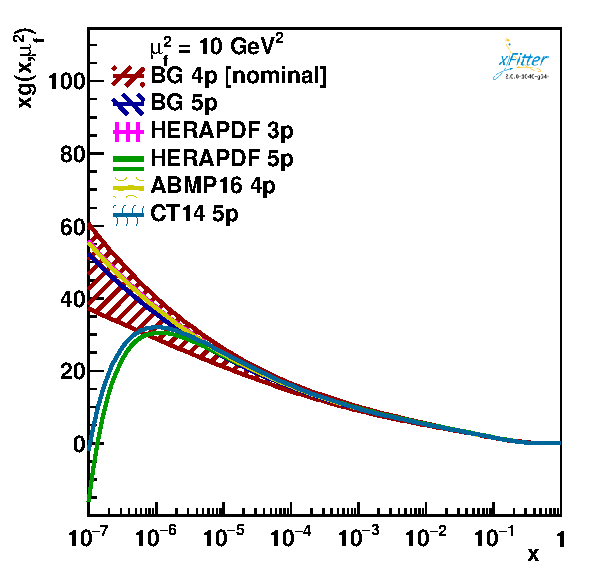
\includegraphics[width=0.49\textwidth]{figs/gluonpar/q2_10_pdf_g.pdf}
    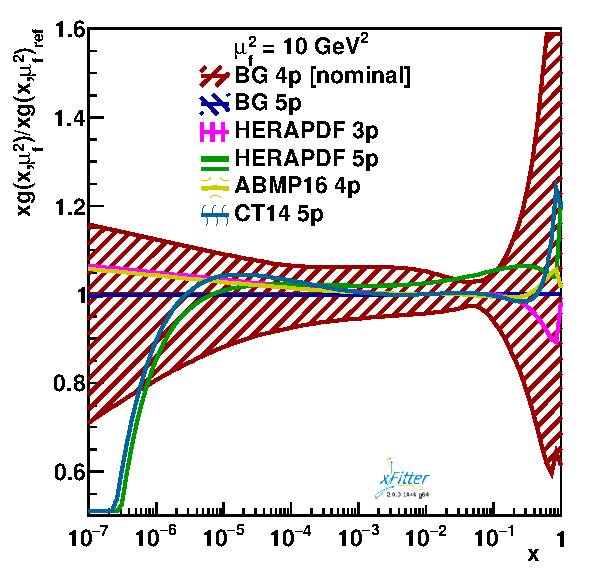
\includegraphics[width=0.49\textwidth]{figs/gluonpar/q2_10_pdf_g_ratio.pdf}
    \caption{(left) The gluon PDF with their total uncertainties at the scale $\mu^2_f=10$ GeV$^2$ obtained using different gluon parametrisations, see Eq.~(\ref{eq:gluonpar}). (right) The same PDFs normalised to the distribution obtained using the nominal parametrisation.}
    \label{fig:gluonpar}
\end{figure}

\section{PDF uncertainties}
\label{sec:pdfunc}

The PDF uncertainties are investigated according to the general approach of HERAPDF2.0 analysis~\cite{Abramowicz:2015mha}, with the fit, model, and parametrisation uncertainties taken into account.

The fit uncertainties arising from the uncertainties in the measurements are estimated by using the Hessian method~\cite{Pumplin:2001ct}, adopting the tolerance criterion of $\Delta \chi^2$ = 1 and correspond to 68\% confidence level.

To investigate the impact of model assumptions on the resulting PDFs, alternative fits are performed and the differences to the central result are considered as model uncertainties. The strangeness fraction is varied as $0.3 \leq f_{s} \leq 0.5$ and the value of $Q^2_{\text{min}}$ imposed on the HERA data as $2.5 \leq Q^2_\textrm{min}\leq 5.0~\textrm{GeV}^2$. The FFNS strong coupling constant is assumed as $0.105 < \alpha_s^{n_f=3}(M_Z) < 0.107$ (corresponding to the VFNS values of $0.117 < \alpha_s^{n_f=5}(M_Z) < 0.119$~\cite{Tanabashi:2018oca}). The variation of the fragmentation parameters $\alpha_K = 4.4 \pm 1.7$ for charm hadrons~\cite{Aaron:2008ac,Chekanov:2008ur} and $\alpha_K = 11 \pm 3$ for beauty hadrons~\cite{Nason:1999zj} is performed.
The scales $\mu_f$ and $\mu_r$ for heavy quark production are varied independently and simultaneously up and down by a factor of two, excluding variations of the two scales in opposite directions. Note that for 
the normalised cross section predictions, the simultaneous variation of the $\mu_f$ and $\mu_r$ scales in the same direction results in the largest deviation in the 
resulting PDFs and is considered as one PDF uncertainty eigenvector.

The parametrisation uncertainty is estimated by extending the functional form of each PDF in Eq.~(\ref{eq:dv}) with additional parameters $D$ and $E$, see Eq.~(\ref{eq:de}), 
which are added or removed one at a time and do not impact the $\chi^2$. 
Furthermore, the shape of the gluon PDF is extended by adding the $+G_g\log^2 x$ term~\cite{Bonvini:2019wxf}. This modification does not result in an improvement in $\chi^2$ and therefore is not considered in the nominal parametrisation. 
The variation of the starting scale, $1.6 < \mu_\mathrm{f0}^2 < 2.2$~GeV$^2$, is also taken into account as contribution to the parametrisation uncertainty. The parametrisation uncertainty is constructed as an envelope built from the maximal differences between the PDFs resulting from all the parametrisation variations and the central fit at each $x$ value.

The total PDF uncertainty is obtained by adding experimental, model, and parametrisation  uncertainties in quadrature.


%\bibliographystyle{h-physrev5}
%\bibliography{prosa2019,extra}
%\end{document}


\section{PROSA 2019 parton distributions}
\label{sec:results}

The quality of the overall fit can be judged based on the global $\chi^2$ divided by the number of degrees of freedom, $n_{dof}$. For each data set included in the fit, a partial $\chi^2$
divided by the number of measurements (data points), $n_{dp}$, is provided. The correlated part of $\chi^2$ quantifies the influence of the correlated systematic uncertainties in the fit. The global and partial $\chi^2$ values for each data set are listed in Table~\ref{tab:chi}, illustrating a general agreement among all the data sets. The central values and the uncertainties of the fitted parameters are given in Table~\ref{tab:pars}.

\begin{table}
\renewcommand*{\arraystretch}{1.12}
\tabcolsep1cm
    \centering
\begin{tabular}{ll}
    Data set & $\chi^2/\textrm{ndp}$ \\
    \hline
    HERA CC $e^{+}p$ & 62 / 39  \\ 
    HERA CC $e^{-}p$ & 49 / 42  \\ 
    HERA NC $e^{-}p$ & 227 / 159  \\ 
    HERA NC $e^{+}p$ 820 GeV & 68 / 70  \\ 
    HERA NC $e^{+}p$ 920 GeV & 440 / 377  \\ 
    HERA NC $e^{+}p$ 460 GeV & 223 / 204  \\ 
    HERA NC $e^{+}p$ 575 GeV & 223 / 254  \\ 
    HERA NC charm & 49 / 52  \\ 
    HERA NC beauty & 18 / 27  \\ 
    LHCb 7 TeV $B^0$ & 52 / 76  \\ 
    LHCb 7 TeV $B^{+}$ & 129 / 108  \\ 
    LHCb 7 TeV $B^{0}_s$ & 37 / 60  \\ 
    LHCb 7 TeV $D^0$ & 15 / 30  \\ 
    LHCb 7 TeV $D^{+}$ & 19 / 29  \\ 
    LHCb 7 TeV $D^{+}_{s}$ & 14 / 20  \\ 
    LHCb 7 TeV $D^{*+}$ & 16 / 22  \\ 
    LHCb 5 TeV $D^0$ & 60 / 35  \\ 
    LHCb 5 TeV $D^{+}$ & 25 / 35  \\ 
    LHCb 5 TeV $D^{+}_{s}$ & 30 / 29  \\ 
    LHCb 5 TeV $D^{*+}$ & 35 / 30  \\ 
    LHCb 13 TeV $D^0$ & 111 / 60  \\ 
    LHCb 13 TeV $D^{+}$ & 72 / 64  \\ 
    LHCb 13 TeV $D^{+}_{s}$ & 69 / 55  \\ 
    LHCb 13 TeV $D^{*+}$ & 82 / 54  \\ 
    ALICE 7 TeV $D^0$ & 5.1 / 8  \\ 
    ALICE 7 TeV $D^{+}$ & 0.75 / 7  \\ 
    ALICE 7 TeV $D^{*+}$ & 2.3 / 6  \\ 
    ALICE 5 TeV $D^0$ & 6.3 / 10  \\ 
    ALICE 5 TeV $D^{+}$ & 5.8 / 9  \\ 
    ALICE 5 TeV $D^{+}_{s}$ & 2.5 / 4  \\ 
    ALICE 5 TeV $D^{*+}$ & 1.7 / 9  \\ 
    \hline
    Correlated $\chi^2$  & 282  \\ 
    Log penalty $\chi^2$  &  -32  \\ 
    \hline
    %\rowcolor{white}
    %\midrule
    Total $\chi^2$ / dof  & 2401 / 1969  \\ 
    %\rowcolor{white}
    %\midrule
    %$\chi^2$ p-value  & 0.00 & 0.00   \\ 
    %\bottomrule
\end{tabular}
\caption{The global and partial $\chi^2$ values for each data set together with the corresponding number of data points (ndp). The correlated $\chi^2$ and the log penalty $\chi^2$ entries refer to the $\chi^2$ contributions from the correlated uncertainties and from the logarithmic term, respectively, as described in Ref.~\cite{Abramowicz:2015mha}.}
\label{tab:chi}
\end{table}

\begin{table}
    \renewcommand*{\arraystretch}{1.12}
    \tabcolsep1cm
    \centering
\begin{tabular}{ll}
    Parameter & Value \\
    \hline
    $B_g$ & $0.004 \pm 0.053$  \\
    $C_g$ & $6.25 \pm 0.29$  \\
    $Fg$ & $0.068 \pm 0.024$  \\
    $B_{u_v}$ & $0.644 \pm 0.030$  \\
    $C_{u_v}$ & $4.862 \pm 0.076$  \\
    $E_{u_v}$ & $15.8 \pm 2.2$  \\
    $B_{d_v}$ & $0.873 \pm 0.076$  \\
    $C_{d_v}$ & $4.61 \pm 0.35$  \\
    $C_{\overline{U}}$ & $7.36 \pm 0.77$  \\
    $D_{\overline{U}}$ & $10.1 \pm 2.4$  \\
    $A_{\overline{D}}$ & $0.1061 \pm 0.0058$  \\
    $B_{\overline{D}}$ & $-0.1661 \pm 0.0062$  \\
    $C_{\overline{D}}$ & $12.7 \pm 3.0$  \\
    $m_c(m_c)$ & $1.230 \pm 0.031$ GeV  \\
    $m_b(m_b)$ & $3.977 \pm 0.100$ GeV  \\
\end{tabular}
\caption{The resulting parameters for the PDFs with their fit uncertainties.}
\label{tab:pars}
\end{table}

The resulting PROSA 2019 PDFs with their total uncertainties at the scale $\mu^2_f=10$ GeV$^2$ are shown in Fig.~\ref{fig:pdfs}. These are compared to the result of the PROSA 2015 fit~\cite{Zenaiev:2015rfa}. In Fig.~\ref{fig:pdfratios} (left), the gluon distribution 
normalised to the one from the PROSA 2015 fit is shown. The two results are in a very good agreement and a significant improvement 
in the precision of the gluon PDF is achieved at $x < 10^{-4}$, as compared to the PROSA 2015 fit. 
The valence and sea quark PDFs are in good agreement with the result of HERAPDF2.0 analysis~\cite{Abramowicz:2015mha} and the 
observed differences in these distributions to the PROSA 2015 analysis are attributed to the update of the DIS measurements~\cite{Aaron:2009aa} used in Ref.~\cite{Zenaiev:2015rfa} to the final combination~\cite{Abramowicz:2015mha} of the HERA data.

The relative total, fit, model and parametrisation uncertainties for the gluon PDF are shown in Fig.~\ref{fig:pdfratios} (right). 
The total uncertainties are dominated by the model uncertainties, with the largest contributions arising from the scale 
variations in predictions for heavy-quark hadroproduction. Reduction of these uncertainties would require theoretical calculations at higher order.  The resulting PDFs are available in the LHAPDF format at the PROSA web-page [https://prosa.desy.de].

\begin{figure}
    \centering
    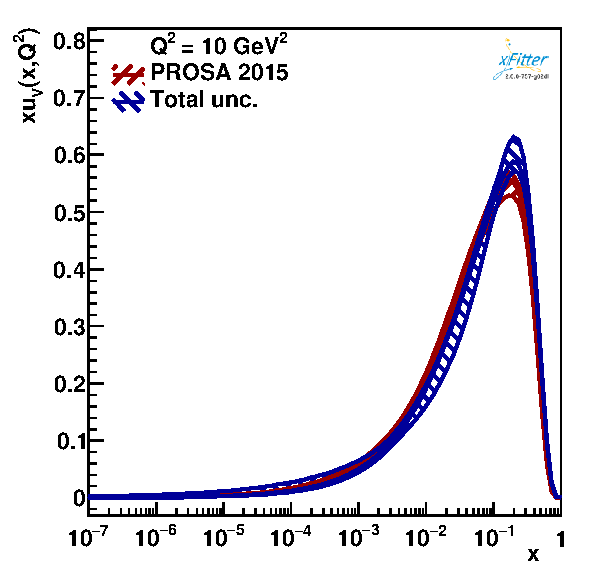
\includegraphics[width=0.49\textwidth]{figs/q2_10_pdf_uv.pdf}
    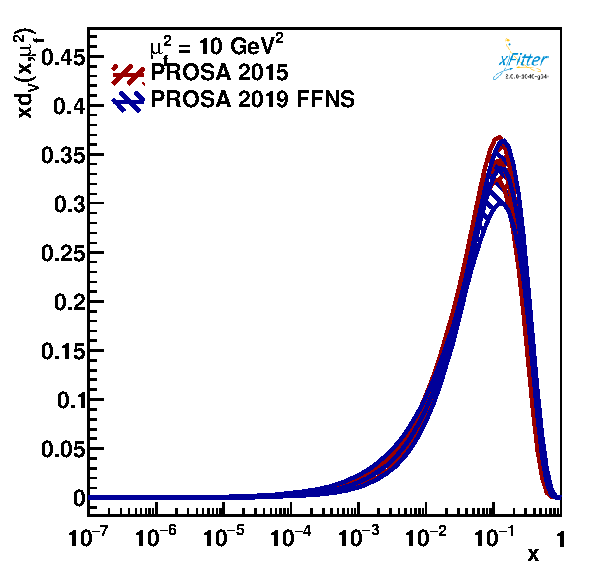
\includegraphics[width=0.49\textwidth]{figs/q2_10_pdf_dv.pdf}\\
    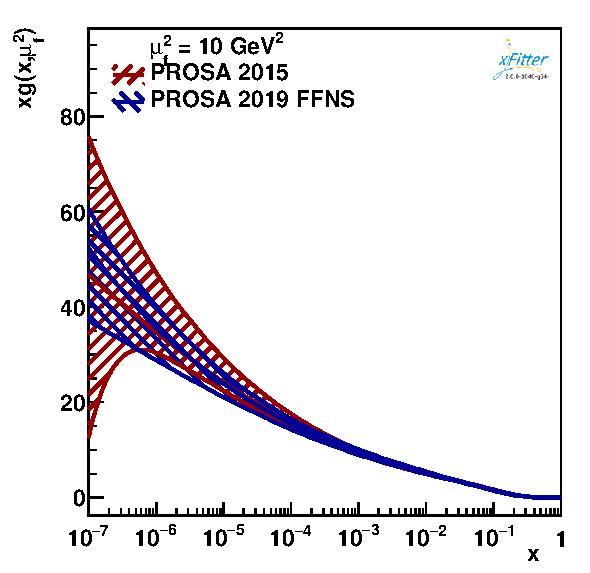
\includegraphics[width=0.49\textwidth]{figs/q2_10_pdf_g.pdf}
    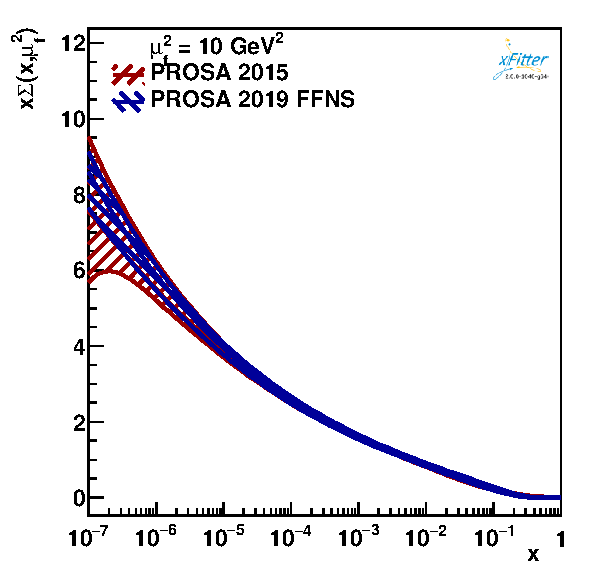
\includegraphics[width=0.49\textwidth]{figs/q2_10_pdf_Sea.pdf}
    \caption{The PROSA 2019 PDF in FFNS with their total uncertainties as a function of $x$ shown at the scale $\mu^2_f=10$ GeV$^2$, compared with the respective distributions from the PROSA 2015 fit.}
    \label{fig:pdfs}
\end{figure}

\begin{figure}
    \centering
    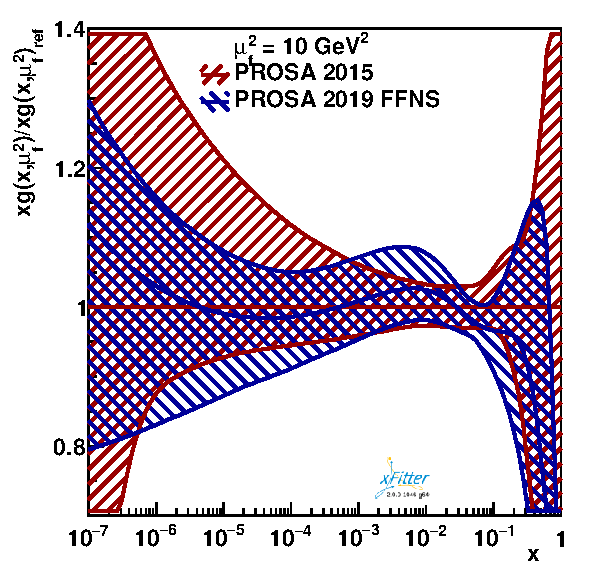
\includegraphics[width=0.49\textwidth]{figs/q2_10_pdf_g_ratio.pdf}
    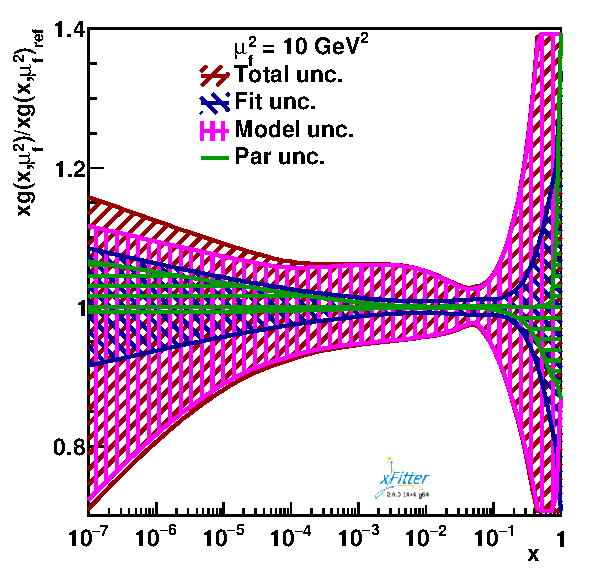
\includegraphics[width=0.49\textwidth]{figs/gluonunc.pdf}
    \caption{Left panel: the ratio of the gluon distributions of PROSA 2019 FFNS and the PROSA 2015, shown as a function of $x$ at the scale $\mu^2_f=10$ GeV$^2$. Right panel: relative total, fit, model and parametrisation uncertainties for the gluon PDF at the scale $\mu^2_f=10$ GeV$^2$.}
    \label{fig:pdfratios}
\end{figure}


\subsection{Fit in VFNS}
\label{sec:vfns}

The fit in the VFNS is performed using the APFEL library~\cite{Bertone:2013vaa} interfaced to xFitter.
The theoretical predictions for the HERA data are computed using the FONLL-B scheme~\cite{Forte:2010ta} with the pole charm and beauty quark masses set to $m_c^{\textrm{pole}} = 1.4$ GeV and $m_c^{\textrm{pole}} = 4.5$ GeV respectively.
However, no VFNS calculation for heavy-quark hadroproduction is interfaced to public QCD analysis tools like xFitter.
To use the MNR calculations with the VFNS, the functionality of the APFEL library is exploited, allowing to choose arbitrary heavy-quark matching thresholds~\cite{Bertone:2017ehk}. These thresholds are set as:
\begin{equation}
\begin{aligned}
\mu_c &= 4.5m_c^{\textrm{pole}} = 6.3~\textrm{GeV},\\
\mu_b &= 4.5m_b^{\textrm{pole}} =  20.25~\textrm{GeV}.
\label{eq:thr}
\end{aligned}
\end{equation}
The kinematic requirements $p_T < 5$ GeV and $p_T < 16$ GeV are imposed on the LHC charm and beauty data, respectively, to ensure that not more than 3 (4) flavours are considered when calculating predictions for charm (beauty) data.
The strong coupling constant is set to $\alpha_s^{n_f = 5}(M_Z) = 0.118$~\cite{Tanabashi:2018oca}, while all other settings are the same as in the FFNS fit.
The specific matching thresholds in Eq.~(\ref{eq:thr}) are chosen to ensure that a sufficient amount of the LHC charm and beauty data is still included in the fit.
The choice of the matching thresholds is arbitrary and coincides with the renormalisation scheme choice~\cite{Bertone:2017ehk}. 
The results are proven to remain stable under variations of $3.1 \le \mu_Q/m_Q^{\textrm{pole}} \le 6$, whereby the $p_T$  cut in the charm and beauty cross section measurements of the LHC are modified accordingly. 

In the VFNS variant of the PDF fit, $\chi^2 = 2114$ is obtained for $n_{dof} = 1714$, indicating a similar quality of data description as compared to the fit in the FFNS. The resulting PDFs are available in the LHAPDF format at the PROSA web-site [https://prosa.desy.de]. No PDF uncertainties are provided with this set.

The performance of the PROSA 2019 VFNS PDFs is tested by computing predictions for the inclusive and multi-jet production in DIS~\cite{Chekanov:2002be,Chekanov:2006xr,Abramowicz:2010cka,Aktas:2007aa,Aaron:2010ac} 
and jet~\cite{Chatrchyan:2012bja} and top quark-antiquark production~\cite{Sirunyan:2017azo,Sirunyan:2019zvx} in $pp$ collisions. The results collected at the PROSA web-site [https://prosa.desy.de] are found similar to those using HERAPDF2.0 PDF.

\section{Predictions for prompt atmospheric neutrino fluxes}
\label{sec:astro}
Various applications in high-energy astroparticle physics could benefit from accurate PDFs in the low-$x$ region. One of the most interesting cases is the evaluation of the atmospheric flux of prompt neutrinos,
%~\cite{Costa:2000jw, Gaisser:2013ira}
originating from the semileptonic decays of heavy-flavoured hadrons produced in the interactions of cosmic rays (CR) with nuclei in the atmosphere. The prompt atmospheric neutrino flux represents the main background for searches of highly energetic
cosmic neutrinos, which are supposed to be produced in the vicinity of far astrophysical sources and in the Galactic Plane~\cite{Gaisser:2016uoy}.  
Such searches are conducted at Very Large Volume Neutrino Telescopes such as ANTARES~\cite{Collaboration:2011nsa}, IceCube~\cite{Gaisser:2014foa} and KM3NeT~\cite{Adrian-Martinez:2016fdl}, which register and analyse the features of the track and cascade events induced by the charged-current and neutral-current weak interactions of the impinging neutrinos with the water/ice nuclei. To date, no direct measurement of the prompt atmospheric neutrino flux is available. Therefore, the most precise theoretical predictions for these fluxes are needed for the reliable interpretation of the experimental data in order to disentangle the cosmic neutrino component from the atmospheric background~\cite{Mascaretti:2019uqn}.

In this paper, the predictions for the prompt atmospheric neutrino fluxes are calculated, in general following the method detailed in Ref.~\cite{Garzelli:2016xmx}. It is assumed, that $pA$ and $AA$ interactions leading to charm production can be described in terms of $pp$ interactions (superposition model) in pQCD. In the present calculation, the proton structure is described by the new PROSA fit, referred to as PROSA 2019.
Production and decay of the $D^\pm$, $D^0$, $\bar{D}^0$, $D_s^\pm$, $\Lambda_c^\pm$ in the atmosphere is considered dominant, 
since the contribution of other charmed hadrons, as well as b-flavoured hadrons, amounts to 5-15\% of the dominant one~\cite{Bhattacharya:2016jce}. In the computation of charmed-hadron production cross sections, the renormalisation and factorisation scales are chosen as $\mu_R$ = $\mu_F$ = $\mu_0$ = $\sqrt{p_T^2 + 4 m_c^2}$, consistent with the scale choice adopted in the theory predictions of $D$- and $B$-meson production at LHCb and ALICE used in the PDF fit. Note that this scale choice differs from the one of Ref.~\cite{Garzelli:2016xmx}, where $\mu_R$ = $\mu_F$ = $\sqrt{p_T^2 + m_c^2}$ was used, consistent with~\cite{Zenaiev:2015rfa}. While the difference between the two scale choices reduces with increasing $p_T$, at low $p_T$, the present scale choice is motivated by faster convergence of the perturbative series to NNLO for the total $pp$~$\rightarrow$~$c\bar{c} + X$ cross section at the LHC energies, as reported in Ref.~\cite{Garzelli:2015psa}. 

In the present work, the central value of the pole mass of the charm quark, $m_c^{pole}$ = 1.43 GeV is used, corresponding to $m_c(m_c) = 1.23$ GeV in the PDF fit (see Table 2), as obtained using 1-loop conversion. It is worthwhile to note that this value is somewhat larger then the one\footnote{In Ref.~\cite{Garzelli:2016xmx}, the $m_c$=1.4 GeV was used instead of the $m_c$=1.25 GeV obtained in the PDF fit of Ref.~\cite{Zenaiev:2015rfa}.} used in Ref.~\cite{Garzelli:2016xmx}. The uncertainty due to the choice of the charm quark mass is evaluated by varying the pole mass by~$\pm$~0.15~GeV around the central value.

The PDF uncertainties are evaluated using the 40 PROSA 2019 uncertainty eigenvectors, accounting for the contributions due to the fit, model, and the parametrisation assumptions. These contributions are then summed up in quadrature. 
The uncertainty related to the choice of the scales is evaluated considering the envelope of the resulting cross section for the assumptions $\mu_R$, $\mu_F$ = \{(1,~1), (0.5,~0.5), (2,~2), (1,~2), (2, 1), (1, 0.5), (0.5, 1)\} ($\mu_0$, $\mu_0$) in the calculation.
  
The predictions for the prompt ($\nu_\mu$ + $\bar{\nu}_\mu$) fluxes are presented in Fig.~\ref{fig1prompt}. Those are obtained by using different hypotheses for the primary CR all-nucleon flux~\cite{Gaisser:2011cc,Gaisser:2013bla}, which are derived from the measured CR all-particle spectrum, under specific assumptions for the CR composition. The QCD uncertainties in the resulting prompt ($\nu_\mu$ + $\bar{\nu}_\mu$) fluxes encompass the uncertainties in the charm quark mass, PDF and those related to the scale choice, with the latter being the dominant uncertainty. As expected, the charm quark mass uncertainty decreases with energy: at small $E_{\nu,\,lab}$ it dominates over the PDF uncertainty, whereas at $E_{\nu,\,lab} \sim 10^7$~-~$10^8$~GeV, both uncertainty contributions become similar. 
At high $E_{\nu,\,lab}$, the PDF uncertainties are reduced with respect to those of Ref.~\cite{Garzelli:2016xmx}, due to 
inclusion of more data sensitive to the low $x$ region in the presented PDF fit. The different contributions of the PDF uncertainty are shown in Fig.~\ref{fig2prompt}. All these contributions increase with increasing $E_{\nu,\,lab}$, which corresponds to the decreasing $x$ of the target parton, probed. 

It is worthwhile to note, that the PDF uncertainties for $E_{\nu,\,lab}$ = $10^6$ - $10^8$ GeV are calculated, assuming the PDFs can
be extrapolated to $x$-values lower than the kinematic reach of the data used in the PDF fit, $x \approx 10^{-6}$.
To date, there are no further measurements probing the $x$-range lower than $10^{-6}$ which would correspond to the highest neutrino energies, which can be accessed~\cite{Goncalves:2017lvq}. However, the result based on PROSA 2019 PDFs reaching the lower $x$ values, remains consistent with the one based on PROSA 2015 PDF set. This fact can be considered as a consistency test of the extrapolation procedure, assuming no New Physics contribution in the probed $x$-range. Furthermore, at the neutrino energies of $E_{\nu,\,lab}~\gtrsim~10^5$ GeV, the assumption on CR composition becomes very important (see Fig.~\ref{fig1prompt}), having an impact on both the shape and the normalisation of the prompt atmospheric neutrino flux.  

In Fig.~\ref{fig3prompt}, the predictions for prompt atmospheric neutrino fluxes are shown. The predictions using FFNS PROSA 2019, PROSA 2015 and ABM11 PDFs with corresponding $\alpha_S(M_Z)$, have been obtained using as a basis matrix-elements for $c\bar{c}$ hadroproduction at NLO in FFNS ($N_f$=3), matched, according to the Powheg formalism~\cite{Nason:2004rx, Frixione:2007nw}, to the {\texttt{PYTHIA8}} Parton Shower and Hadronisation algorithms~\cite{Sjostrand:2014zea}. The predictions using PROSA 2019 PDF at high energies are somewhat lower than those using PROSA 2015 and ABM11 PDFs, due to a somewhat suppressed gluon at low $x$. 
In the same Figure, the predictions obtained in the generalised-mass VFNS framework of Ref.~\cite{Benzke:2017yjn}, using as input 
VFNS PDFs (CT14nlo and the PROSA 2019 VFNS) are shown. The NLO QCD corrections are included in the partonic cross section, whereas the transition from partons to hadrons is described by fragmentation functions evolving with the factorisation scale~\cite{Kneesch:2007ey}, 
a procedure which resums logarithms of $p_T/m_c$ at next-to-leading-logarithmic accuracy. The central predictions using the GM-VFNS are 
compatible among each other, but show shape differences with respect to the FFNS ones. Part of these differences are related to 
the different treatment of the transition of partons into hadrons (parton shower + hadronisation on the one hand, vs. fragmentation 
functions on the other hand). Also, a different factorisation scale is used in the GM-VFNS predictions~\footnote{Motivations for the specific $\mu_F$ = $\mu_R$/2 choice adopted in the GM-VFNS computation are reported in Ref.~\cite{Benzke:2017yjn} }. For comparison, the upper limit on the prompt neutrino flux obtained in the IceCube analysis~\cite{Aartsen:2016xlq} of up-going muons 
from the northern hemisphere is also shown and is well described by the predictions. 


In Fig.~\ref{fig4prompt} the presented flux prediction is compared to those obtained by other groups. In general, all the flux predictions are consistent within the uncertainties. The result of Ref~\cite{Gondolo:1995fq} shows largest differences with the presented result 
due to using the charm cross section calculation at LO only. The ERS dipole model prediction~\cite{Enberg:2008te}, that is mostly used by the experimental collaborations in their data analysis, is also consistent with the prediction of this paper, within uncertainties. The uncertainties in the ERS prediction are smaller compared to the QCD-based prediction, however the way of the uncertainty estimate in both calculations can not be directly compared. Indeed the dipole approach is expected to effectively resum logarithmic contributions of the form $\alpha_S\mathrm{ln}(1/x)$ in the PDF evolution, a property which could lead to a reduction of the PDF uncertainties associated to the target parton at low $x$, whereas the resummation of these logarithms is not included in the DGLAP evolution.
The uncertainties associated to the projectile parton distributions in Ref~\cite{Enberg:2008te} were estimated by comparing 
two different central PDF sets, without considering the PDF uncertainty associated to each of those. Furthermore, the 
factorisation scale variation in Ref.~\cite{Enberg:2008te} is performed in a limited range of $\mu_F$= $m_c$, $\mu_F$=2 $m_c$.

In Fig.~\ref{fig5prompt}, the prediction for the prompt neutrino flux based on the superposition model for both the projectile 
CR and the target nucleon of the air, obtained using the PROSA 2019 PDF set, is compared to the calculation of Ref.~\cite{Bhattacharya:2016jce} which uses nuclear PDFs to describe the target nucleon (nitrogen) and the proton PDFs for the projectile CR. Both predictions agree well with each other.

\begin{figure}
    \centering
    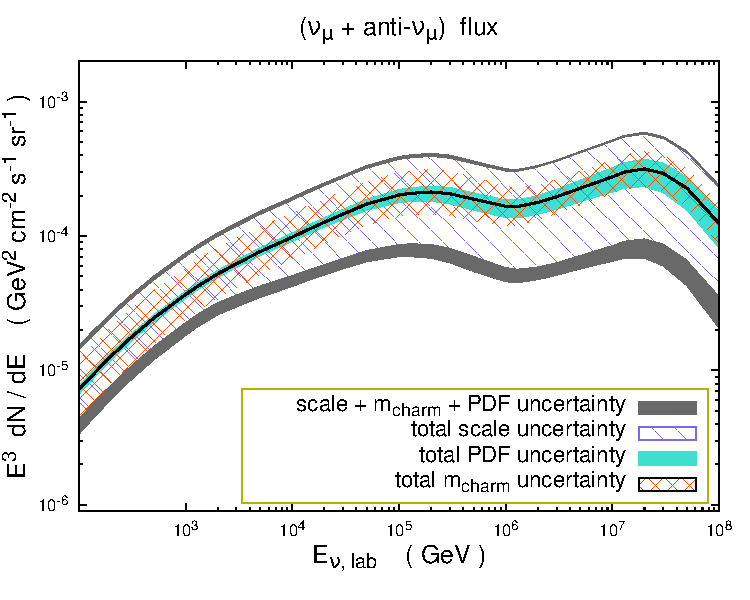
\includegraphics[width=0.49\textwidth]{figs/scalemasspdfunc_prosa19_spettro1_py8.pdf}
    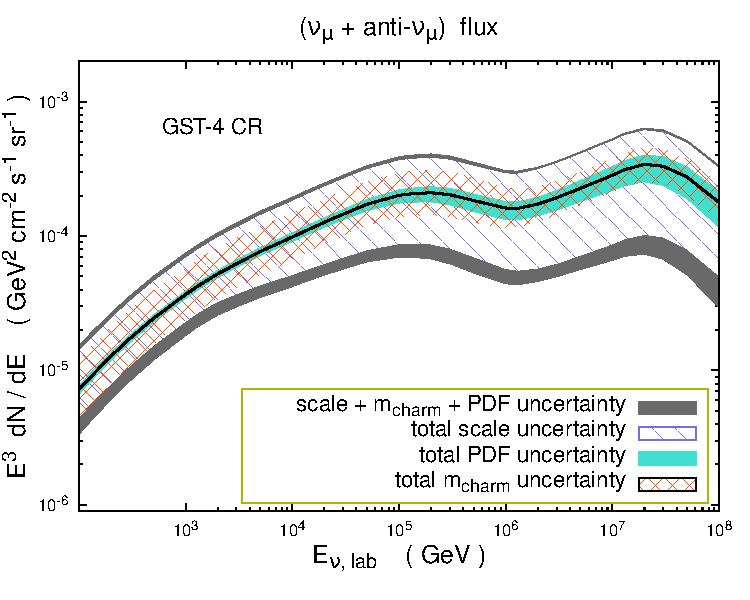
\includegraphics[width=0.49\textwidth]{figs/scalemasspdfunc_prosa19_spettro2_py8.pdf}
    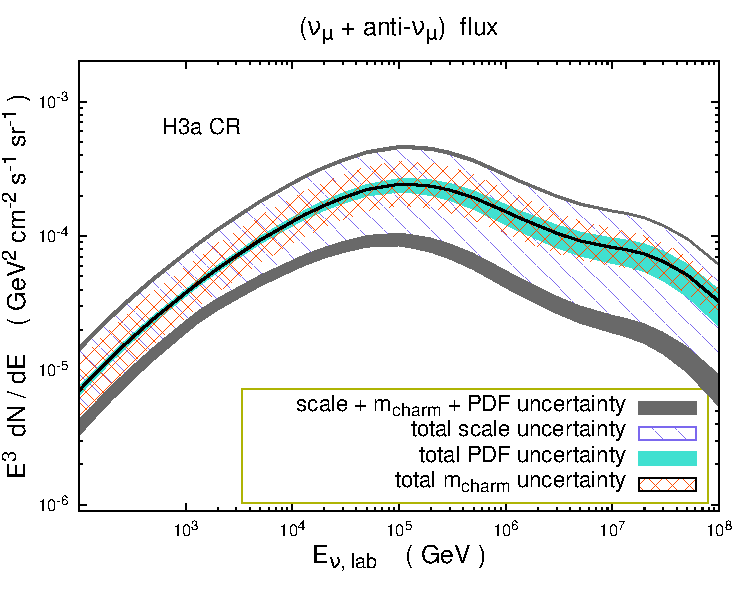
\includegraphics[width=0.49\textwidth]{figs/scalemasspdfunc_prosa19_spettro3_py8.pdf}
    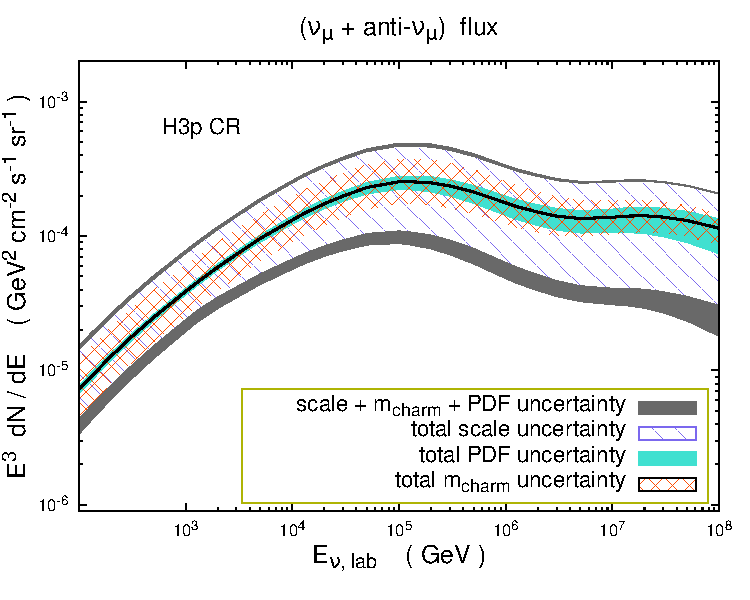
\includegraphics[width=0.49\textwidth]{figs/scalemasspdfunc_prosa19_spettro4_py8.pdf}
    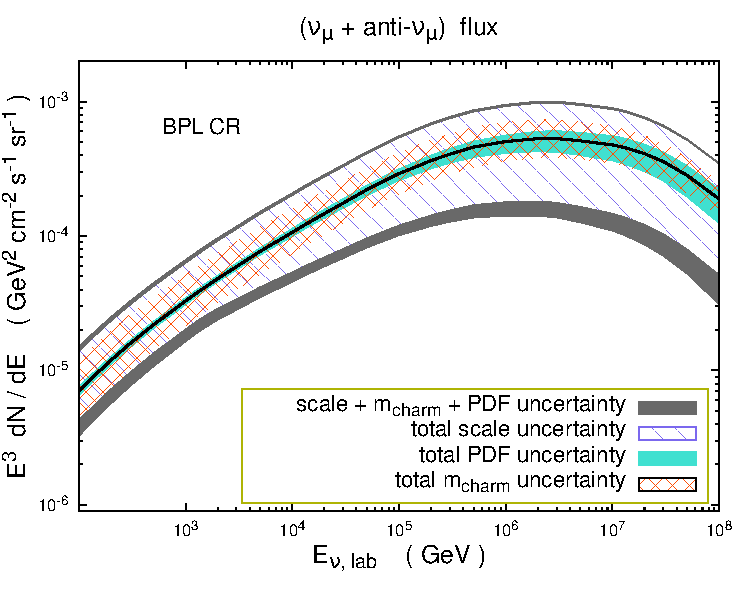
\includegraphics[width=0.49\textwidth]{figs/scalemasspdfunc_prosa19_spettro0_py8.pdf}
    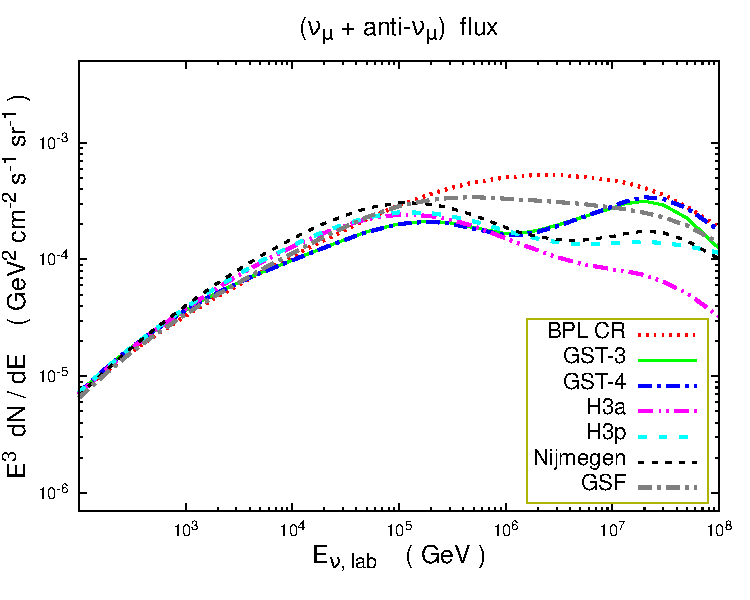
\includegraphics[width=0.49\textwidth]{figs/numuantinumuflux_crfluxvar_spettro01234_pair1_prosa19.pdf}
  \caption{\label{fig1prompt}  Predictions for the prompt atmospheric neutrino fluxes and their uncertainties related to scale variation, charm mass and PDF uncertainties. As CR primary all-nucleon spectra, the GST-3, GST-4, H3p, H3a and BPL are chosen~\cite{Gaisser:2013bla, Gaisser:2011cc}. The central predictions using different primary all-nucleon spectra, are also compared to each other and to together with those obtained using Nijmegen~\cite{Thoudam:2016syr} and GSF~\cite{Dembinski:2017zsh}, each represented by a line of different style.}
\end{figure}


%\begin{figure}
%  \caption{\label{fig2prompt} Central predictions for prompt neutrino fluxes using different CR primary all nucleon spectra, corresponding to different 
%hypotheses for the CR composition.}
%\end{figure}

\begin{figure}
\centering
    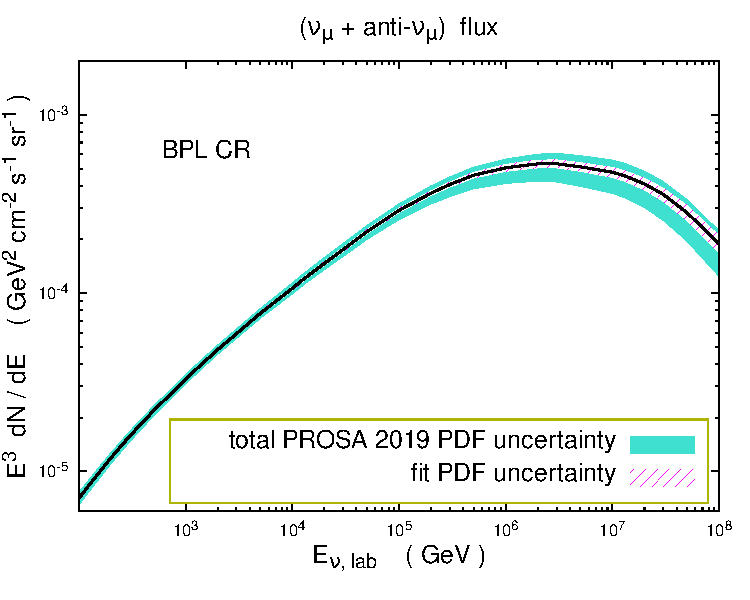
\includegraphics[width=0.49\textwidth]{figs/pdfunc_prosa19_fit_py8.pdf}
    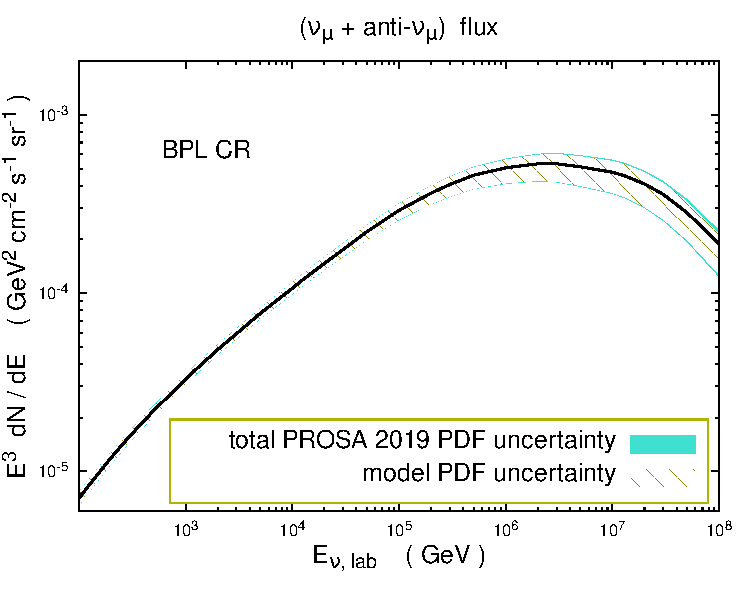
\includegraphics[width=0.49\textwidth]{figs/pdfunc_prosa19_model_py8.pdf}
    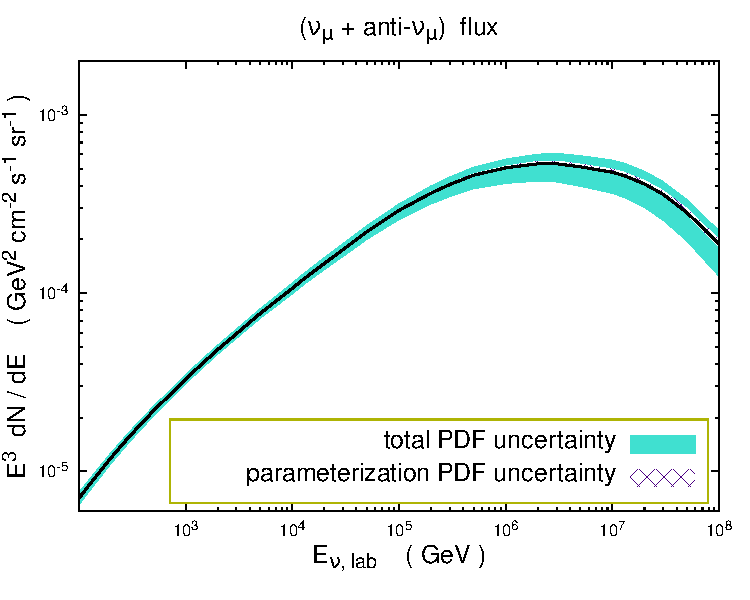
\includegraphics[width=0.49\textwidth]{figs/pdfunc_prosa19_param_py8.pdf}
\caption{\label{fig2prompt} Contributions of the PDF fit, model and parametrisation uncertainties to the total uncertainties in the prediction for the prompt atmospheric neutrino flux using the BPL primary CR all-nucleon spectrum.}  
\end{figure}


\begin{figure}
\centering
    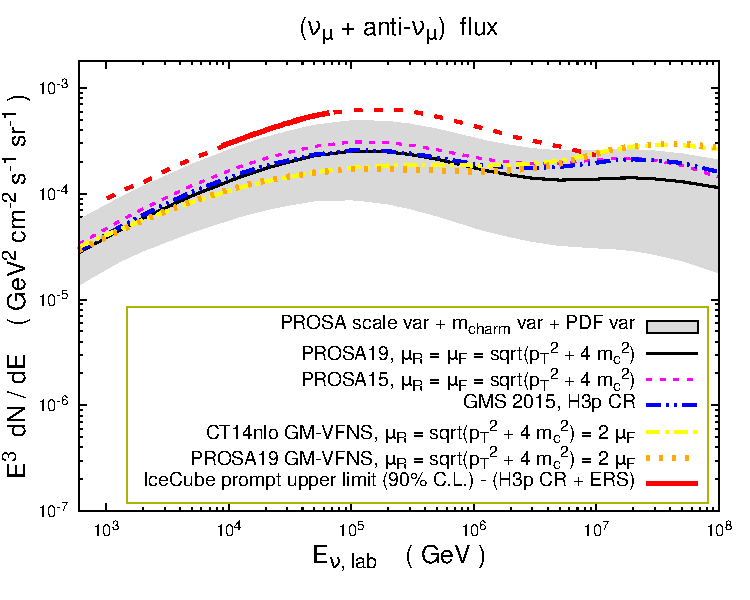
\includegraphics[width=0.62\textwidth]{figs/fluxcompa_prosa19abmmicicecube_verynew2_py8.pdf}
  \caption{\label{fig3prompt} Predictions for prompt atmospheric neutrino fluxes as a function of neutrino energies in FFNS and VFNS using different PDFs in the corresponding scheme, shown by lines of different styles. The experimental upper limit on the prompt atmospheric ($\nu_\mu$ + $\bar{\nu}_\mu$) flux, reported~\cite{Aartsen:2016xlq} by the IceCube collaboration is also shown.}
\end{figure}


\begin{figure}
\centering
    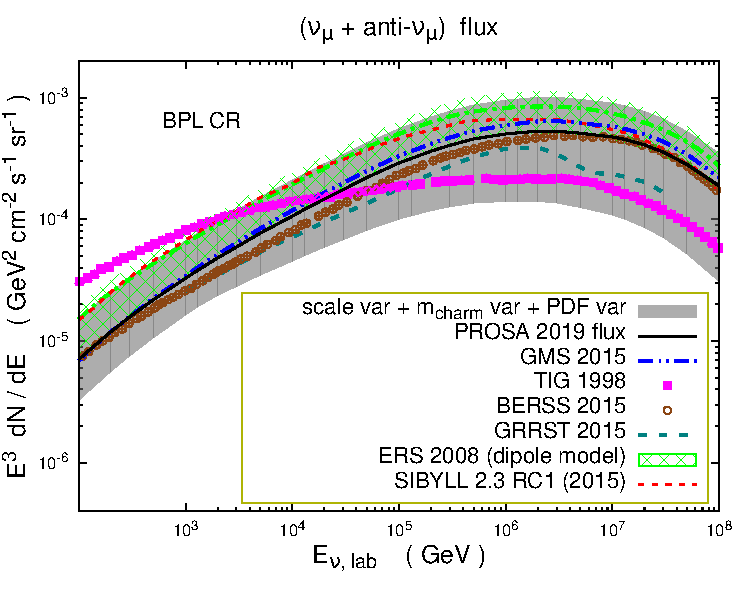
\includegraphics[width=0.7\textwidth]{figs/fluxcompa1_extended_prosa19_py8.pdf}
  \caption{\label{fig4prompt} Predictions for prompt atmospheric neutrino fluxes obtained in the presented analysis, compared to those by other authors~\cite{Garzelli:2015psa, Gondolo:1995fq, Enberg:2008te, Bhattacharya:2015jpa, Gauld:2015kvh, Fedynitch:2015zma}, presented by lines of different style. The primary CR all-nucleon flux BPL is used in all the predictions.}
\end{figure}

\begin{figure}
\centering
    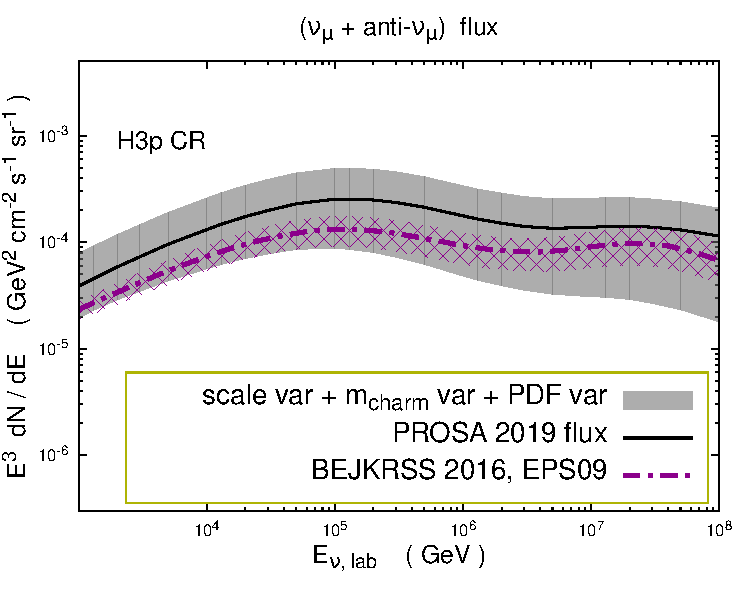
\includegraphics[width=0.49\textwidth]{figs/fluxcompa_prosa19nuovibatta1_py8.pdf}
    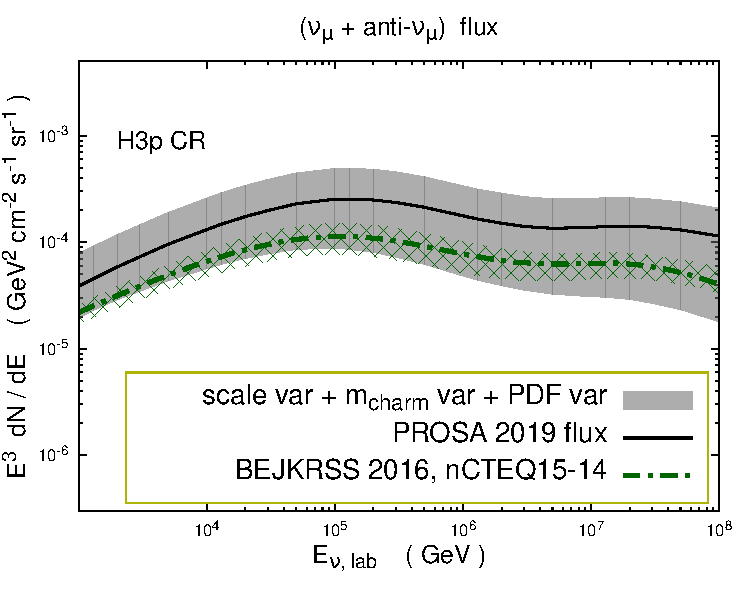
\includegraphics[width=0.49\textwidth]{figs/fluxcompa_prosa19nuovibatta2_py8.pdf}
  \caption{\label{fig5prompt} Predictions for prompt atmospheric neutrino fluxes obtained in the presented analysis, compared to those by other authors~\cite{Bhattacharya:2016jce}. The all-nucleon flux H3p CR is used in all predictions. For the description of the Nitrogen (air) target, the nuclear PDFs EPS09~\cite{Eskola:2009uj} and nCTEQ15~\cite{Kovarik:2015cma} are used.}
\end{figure}

%\bibliographystyle{h-physrev5}
%\bibliography{prosa2019,extra}
%\end{document}


\section{Summary}
\label{sec:summary}

In this paper, the new improved constraints on the parton distributions are presented, as obtained in a QCD analysis at NLO using the DIS and $pp$ collision data. In particular the recent measurements of the LHCb and ALICE experiment of hadroproduction of charm and beauty-flavoured hadrons in the forward kinematic range provide additional sensitivity to the gluon distribution.
Using as a basis different PDF parametrisations, the sensitivity of the results of the fit to the gluon parametrisation used as an input is shown, which is particularly interesting for low $x$'s.  
%at low $x>10^{-6}$.
The PDFs are extracted in FFNS and VFNS and are used to obtain improved predictions for the prompt atmospheric neutrino fluxes. 
We foresee as well their use for further high-energy astrophysical applications, like e.g. the computation of the $nu$-N deep-inelastic-scattering cross-section. At low $x$, the PROSA 2019 fit leads to a gluon PDF somehow suppressed with respect to the PROSA 2015 fit, which leads to a slight decrease of the prompt neutrino fluxes at high energies. An additional factor decreasing the predictions for prompt neutrinos at all energies is represented by the use of a new charm mass value in their computation, consistent with the charm mass value extracted within the PROSA 2019 fit, which turns out to be well compatible with the PDG value.  The PROSA 2019 and the PROSA 2015 predictions remain in any case very well compatible within the uncertainty bands, also reflecting the fact that the PROSA 2015 and PROSA 2019 gluon PDFs are still compatible within the uncertainty bands.  The PROSA 2019 predictions on prompt neutrino fluxes are also compatible within uncertainty with other ones, using nuclear PDFs (instead of the $pp$ superposition model) and with the IceCube experimental upper limit on prompt neutrinos. 


\section*{Acknowledgements}

We would like to thank I.~Novikov and A.~Glazov for their help with developing and using new features of the xFitter framework, and V.~Bertone for his help with the APFEL library. We are grateful to M.~Benzke for having produced the predictions for $D$-meson hadroproduction used as a basis for the computation of prompt neutrino fluxes in the GM-VFNS framework. We thank S. Alekhin for useful discussions and comments. The work of O.~Z. has been supported by Bundesministerium f\"ur Bildung und Forschung (contract 05H18GUCC1).

The authors are grateful to the Mainz Institute for Theoretical Physics (MITP)
of the DFG Cluster of Excellence PRISMA+ (Project ID 39083149), for its
hospitality and its partial support during the completion of this work.


%%%%%%%%%%%%%%%%%%%%%%%%%%%%%%%%%%%%%%%%%
%%%%%%%%%%%%%%%%%%%%%%%%%%%%%%%%%%%%%%%%%

\clearpage
%\bibliographystyle{JHEP}
\bibliographystyle{h-physrev5}
\bibliography{prosa2019,extra}


\end{document}


